% \input{content/Z-Anhang-01-Herleitungen}
\chapter{Datenblatt Hokuyo Laserscanner}
\label{anh:datasheet}
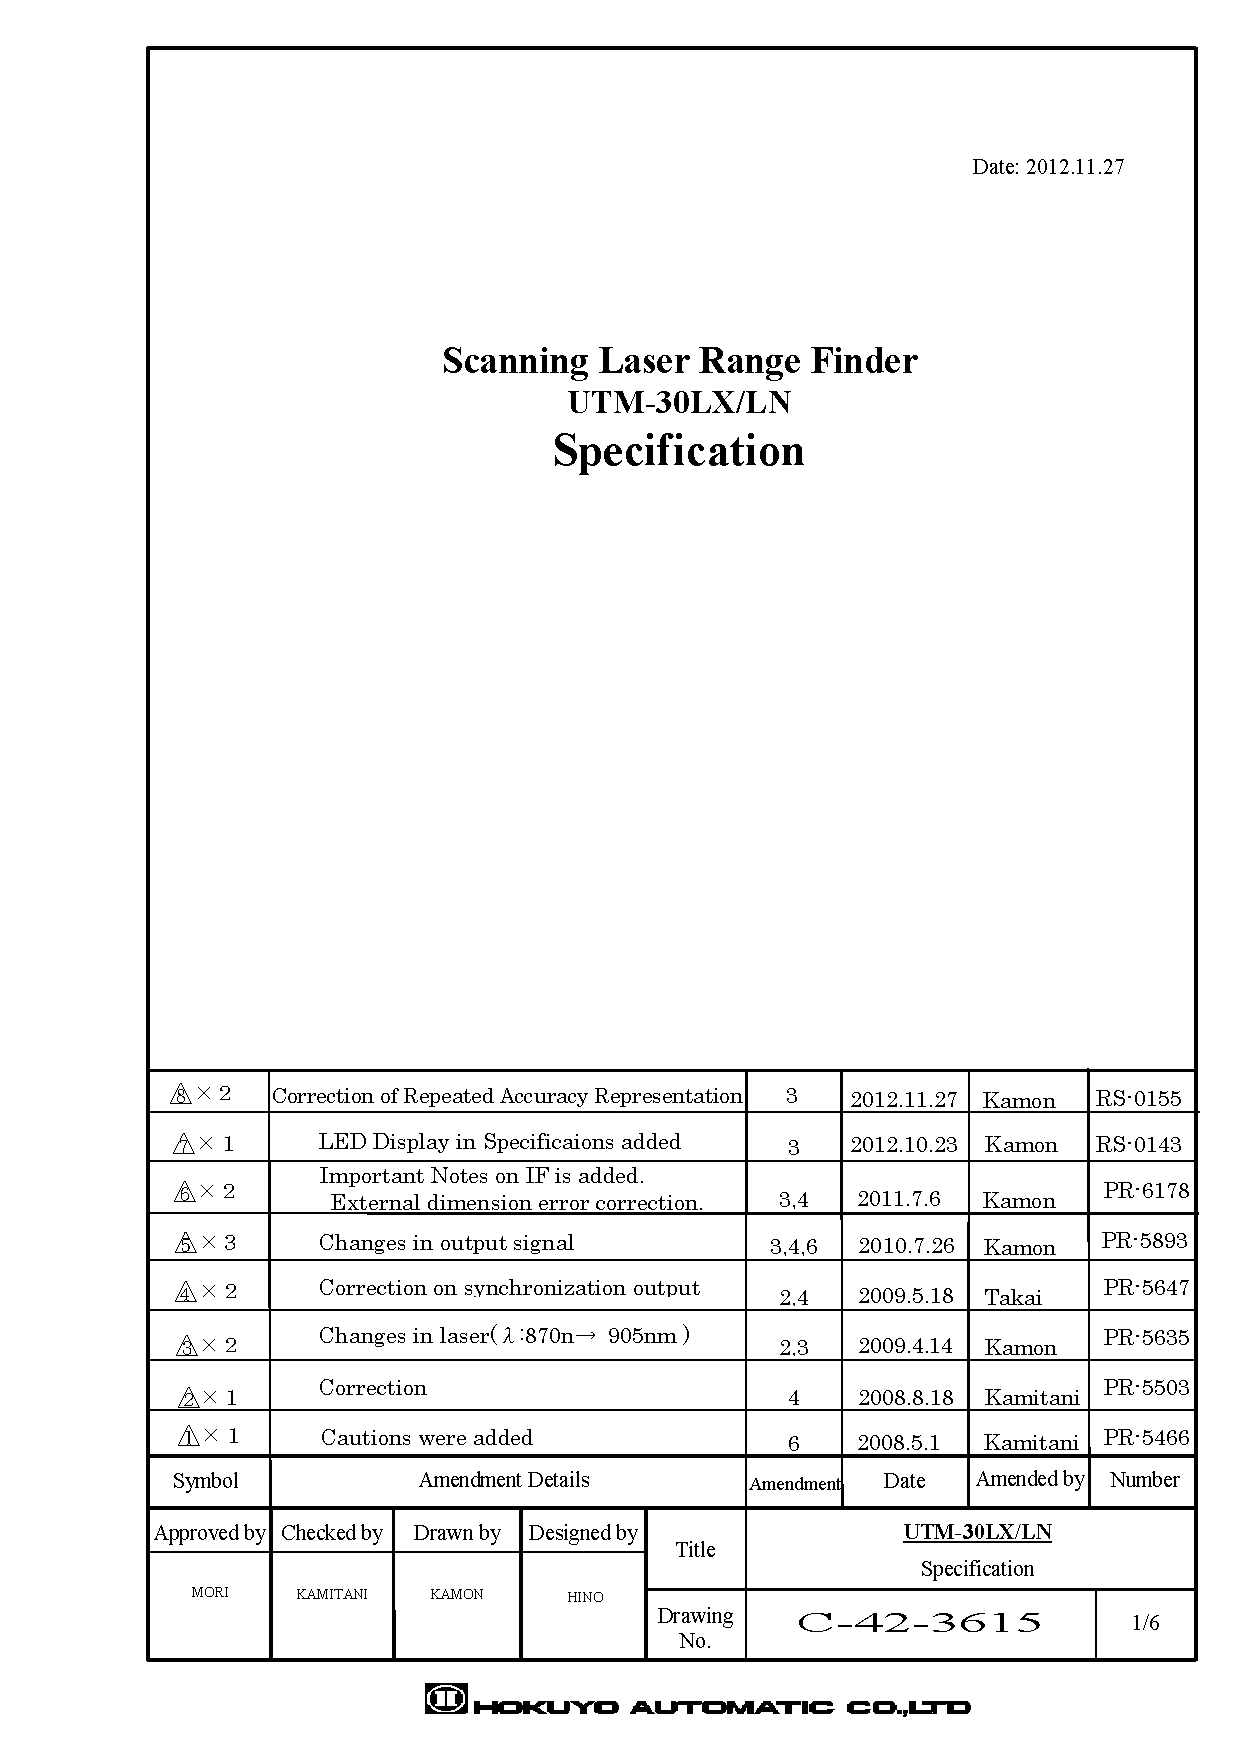
\includepdf[pages=-]{Anhang/UTM_30LX_spec_en}

\chapter{Definition flacher Mehrgr��ensysteme}
\label{anh:def_fl}
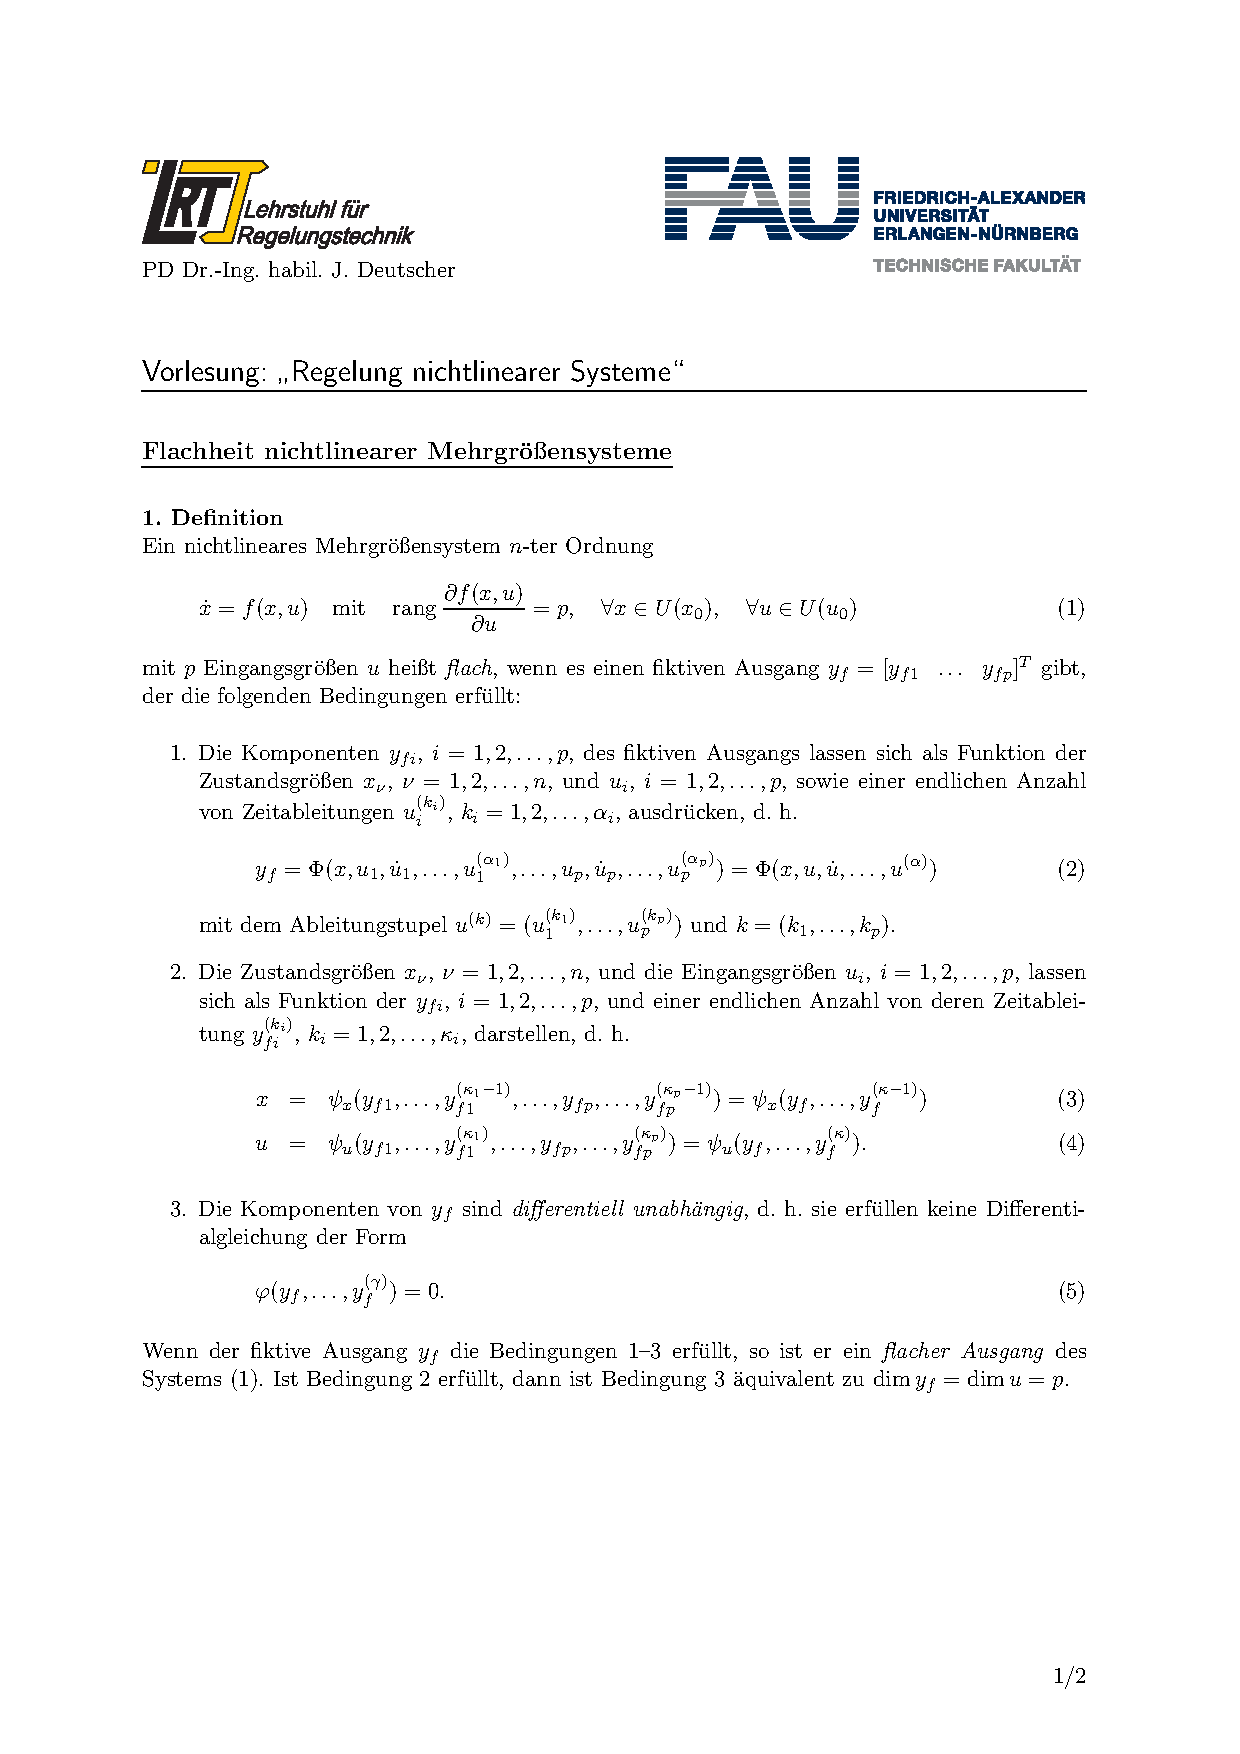
\includepdf[pages=-]{Anhang/Definition_flacher_Mehrgrosensysteme}

\chapter{Simulinkmodell}
\label{anh:simulink}

\section{Gesamt�bersicht Positionsregelung}
%  \begin{figure}
  	\centering
  	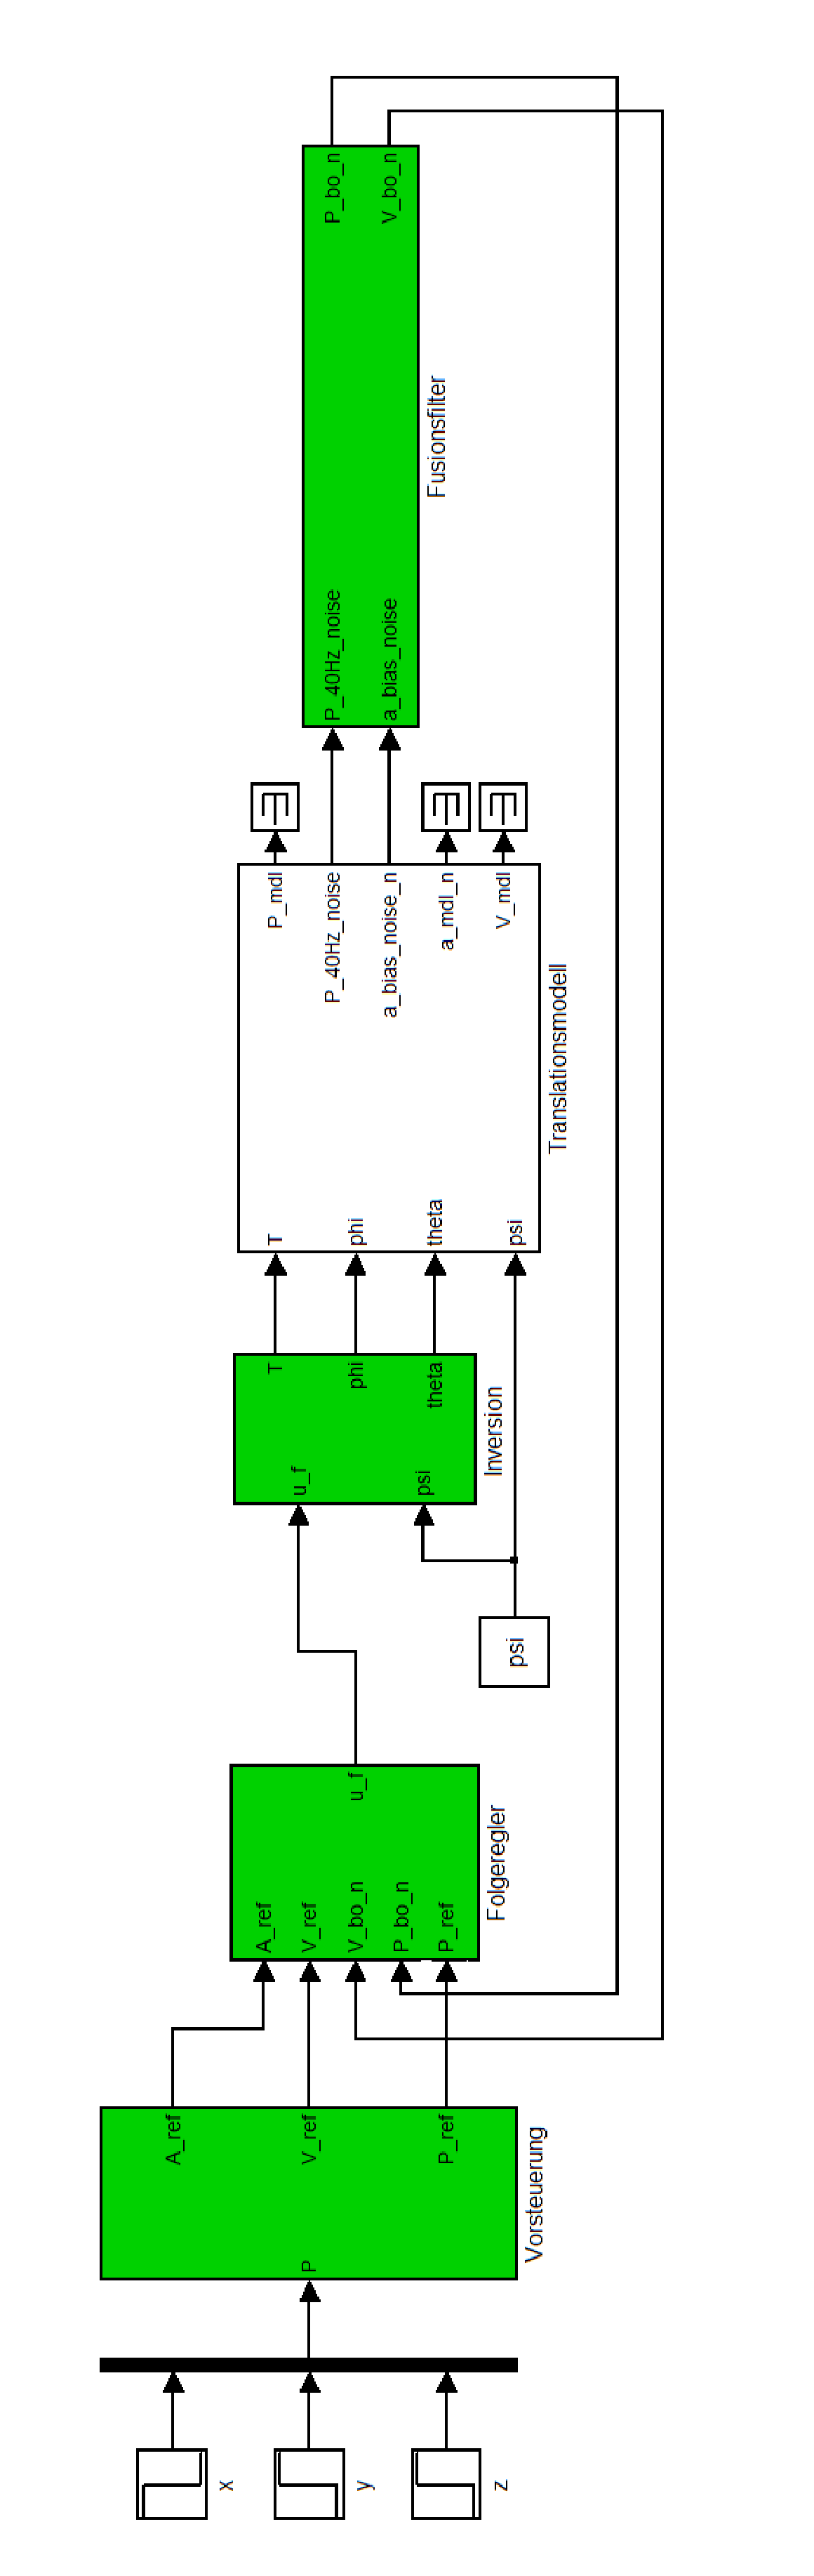
\includegraphics[height = .9\textheight]{images/anlag_gesamtsystem}
 % 	\caption[End-fit \gls{foaw}]{End-sadfsadfasdfsdfasdfit \gls{foaw}} %
  %	\label{fig:foadssdfsdfsadfw}
%  \end{figure}
\section{Translationsmodell}
	\centering
	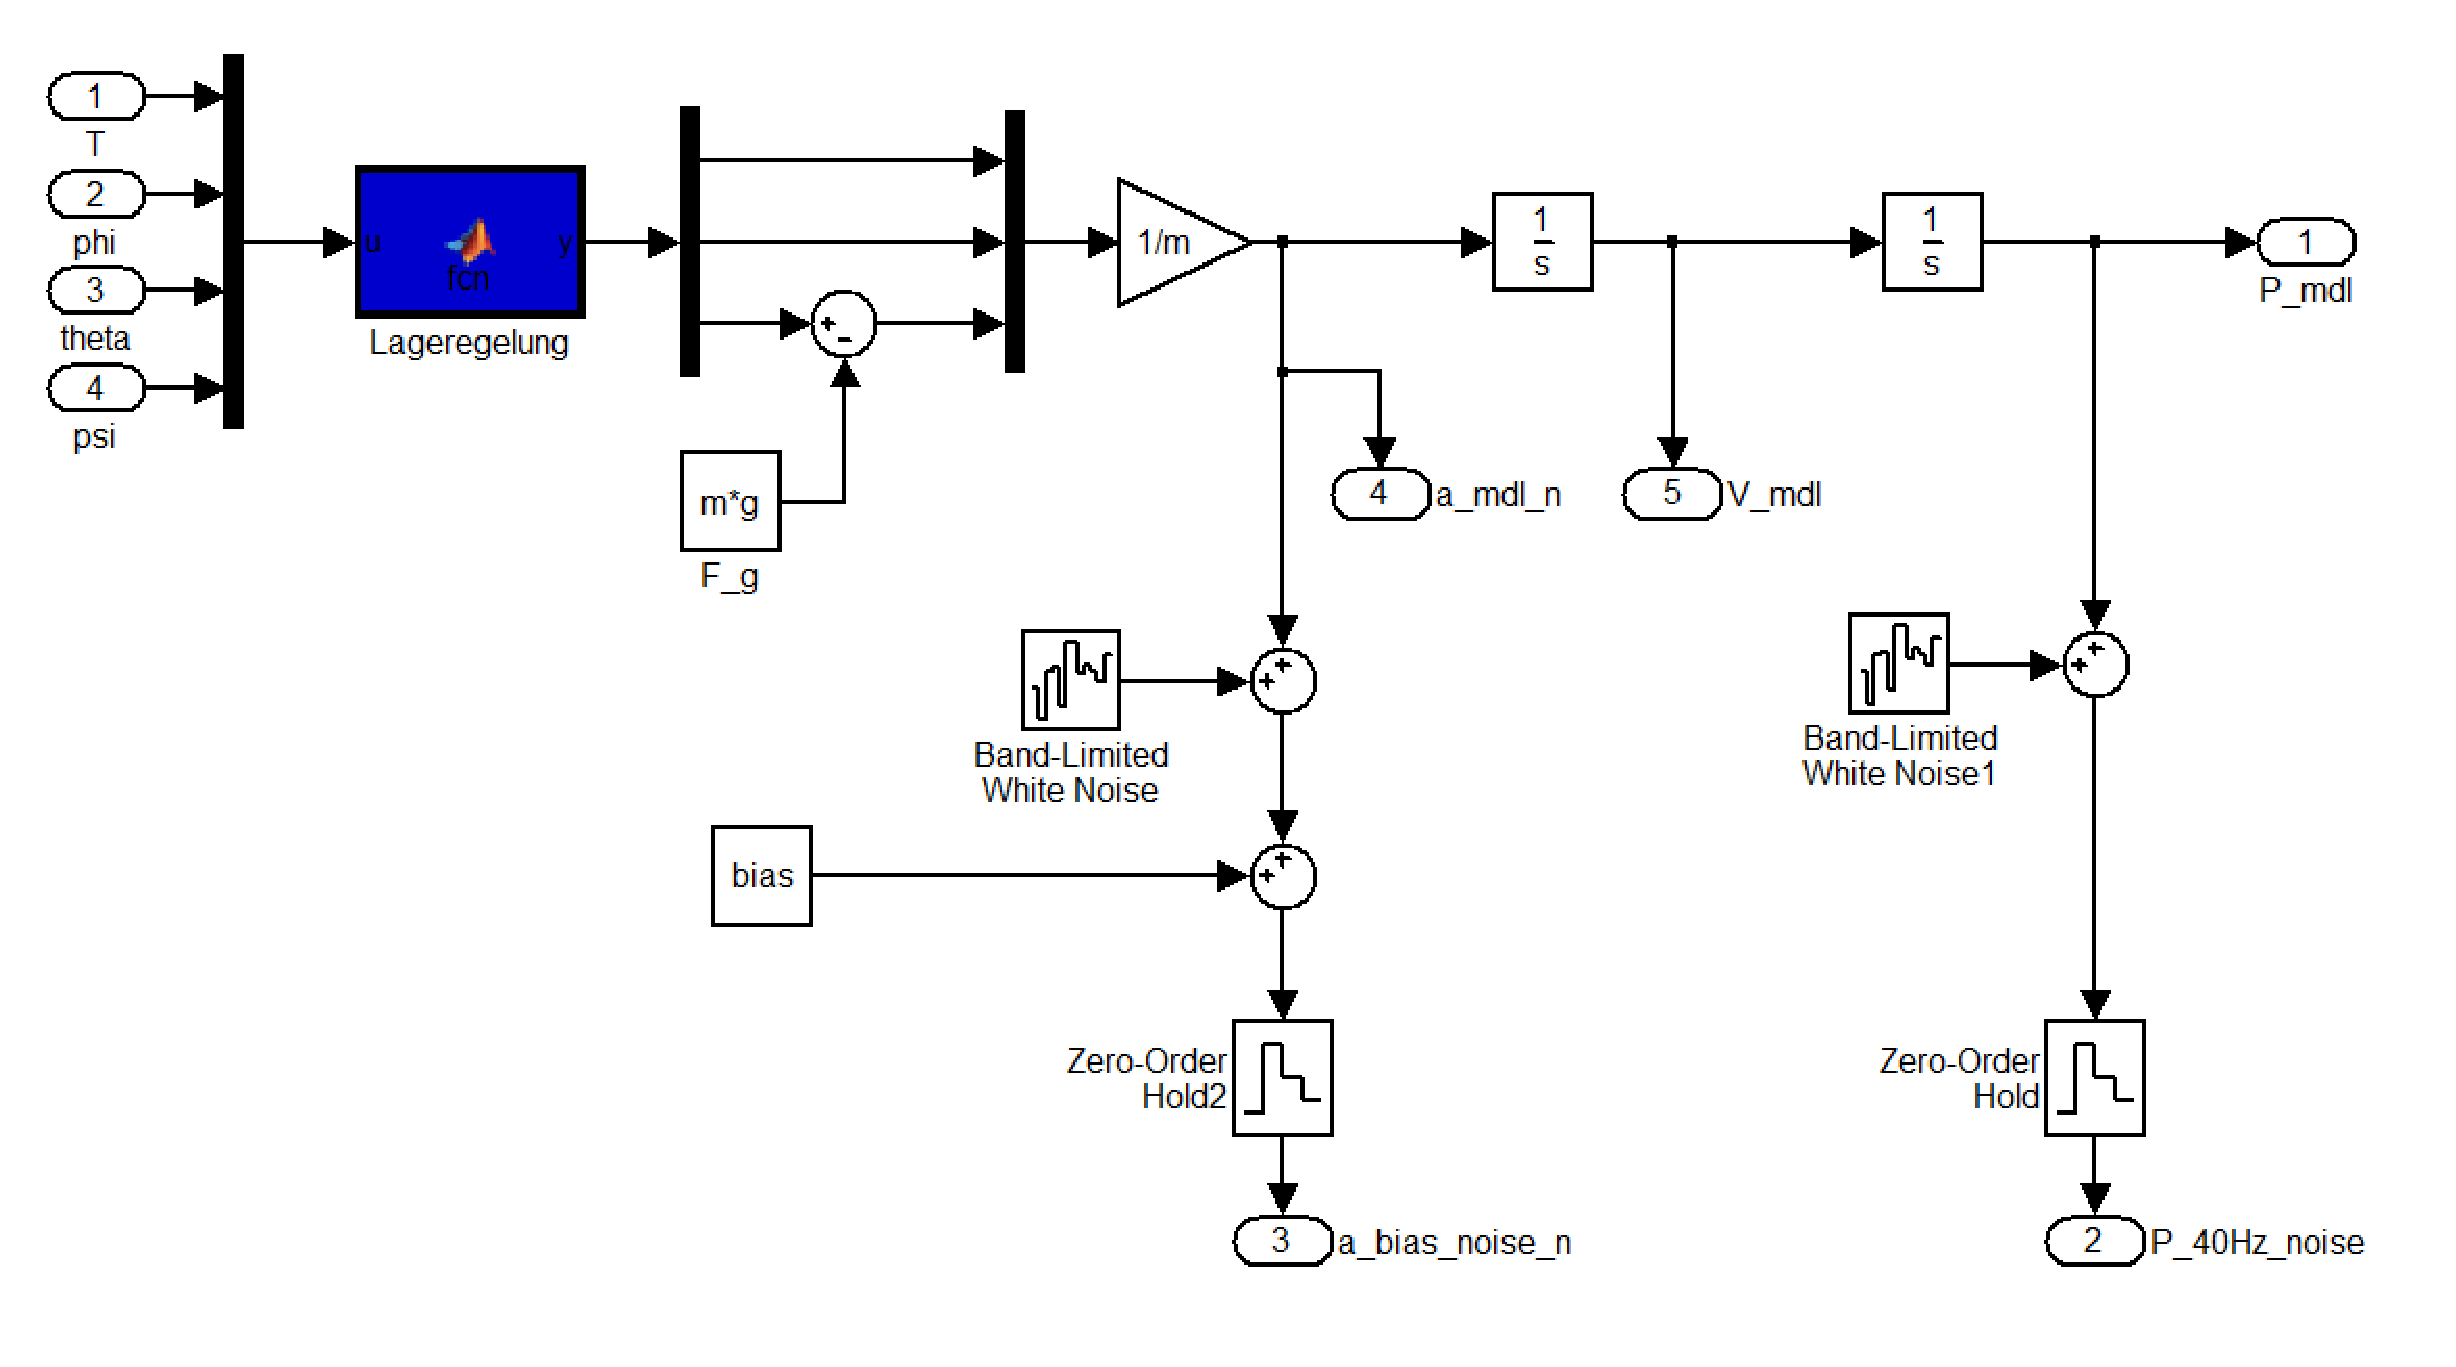
\includegraphics[width = \textwidth]{images/anlag_Translationsmodell}

 \begin{itemize}
 	\item Lageregelung
 	 \begin{lstlisting}
 	 function y = fcn(u)
 	 T       = u(1);
 	 phi     = u(2);
 	 theta   = u(3);
 	 psi     = u(4);
 	 
 	 Mt = [cos(theta) * cos(psi) sin(phi) * sin(theta) * cos(psi) - cos(phi) * sin(psi) cos(phi) * sin(theta) * cos(psi) + sin(phi) * sin(psi); cos(theta) * sin(psi) sin(phi) * sin(theta) * sin(psi) + cos(phi) * cos(psi) cos(phi) * sin(theta) * sin(psi) - sin(phi) * cos(psi); -sin(theta) sin(phi) * cos(theta) cos(phi) * cos(theta);];
 	 y = Mt * [0; 0; T];
 	 \end{lstlisting}
 \end{itemize}

\section{Modell der Inversion}

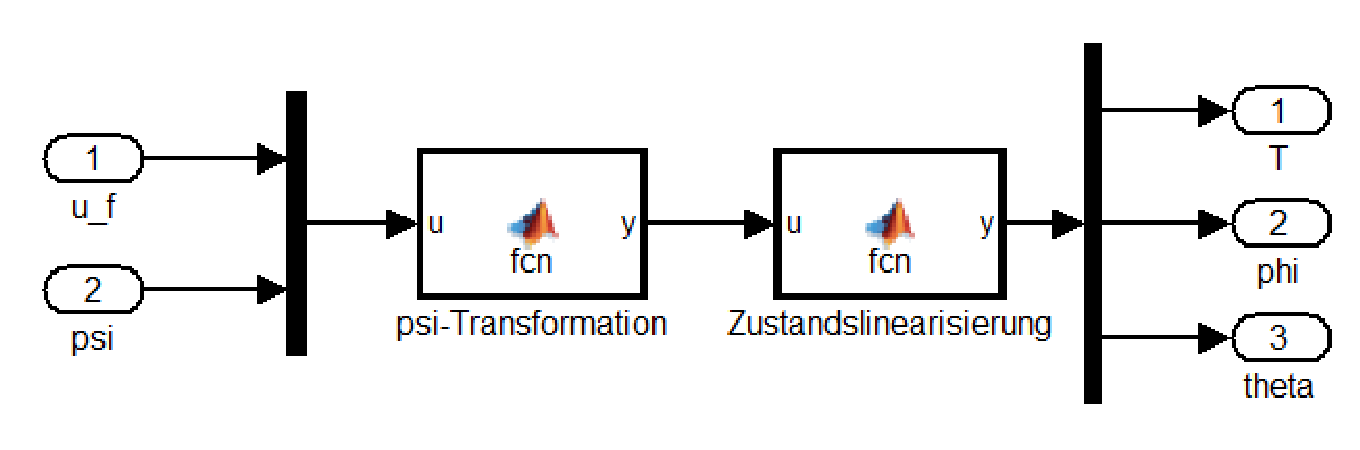
\includegraphics[width = .8\textwidth]{images/anlag_inversion}

 \begin{itemize}
 	\item $ \psi $-Transformation
 	\begin{lstlisting}
 	function y = fcn(u)
 	a_nx = u(1);
 	a_ny = u(2);
 	a_nz = u(3);
 	psi  = u(4);
 	
 	Mz = [cos(psi) sin(psi) 0; -sin(psi) cos(psi) 0; 0 0 1;];
 	y = Mz * [a_nx;a_ny;a_nz];
 	\end{lstlisting}
 	\item Zustandslinearisierung
 	\begin{lstlisting}
	 function y = fcn(u)
	 a_ox = u(1);
	 a_oy = u(2);
	 a_oz = u(3);
	 m = 1.863;
	 g = 9.81;
	 
	 T       = m*(sqrt(a_ox^2+a_oy^2+(a_oz+g)^2));
	 phi     = asin(-(a_oy*m)/T);
	 theta   = atan(a_ox/(a_oz+g));
	 
	 y = [T;phi;theta];
 	\end{lstlisting}
 \end{itemize}
 
 \section{Modell der Vorsteuerung}
 
 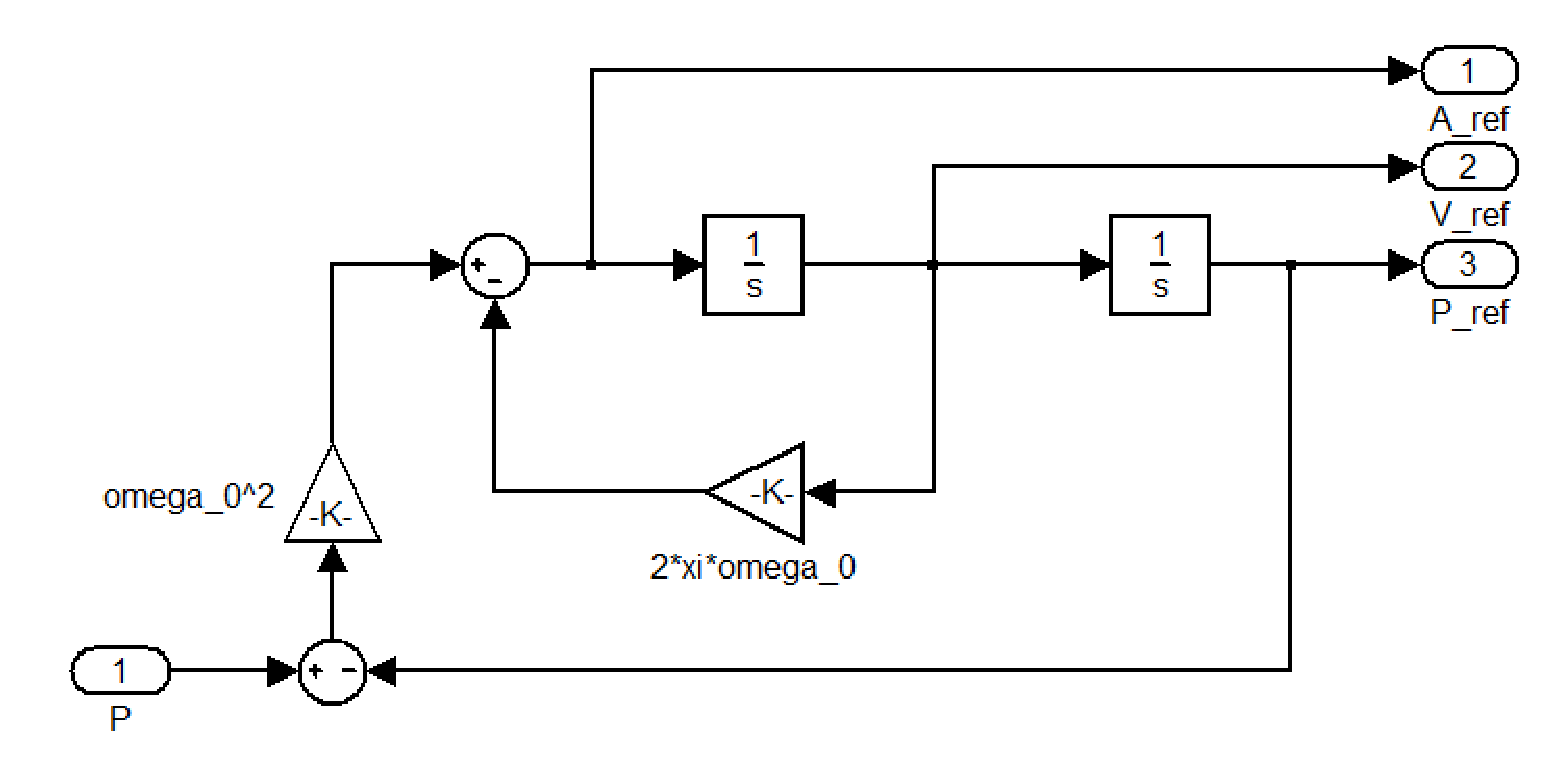
\includegraphics[width = .95\textwidth]{images/anlag_vorsteuerung}
  
 \section{Modell der Folgeregelung}
  
  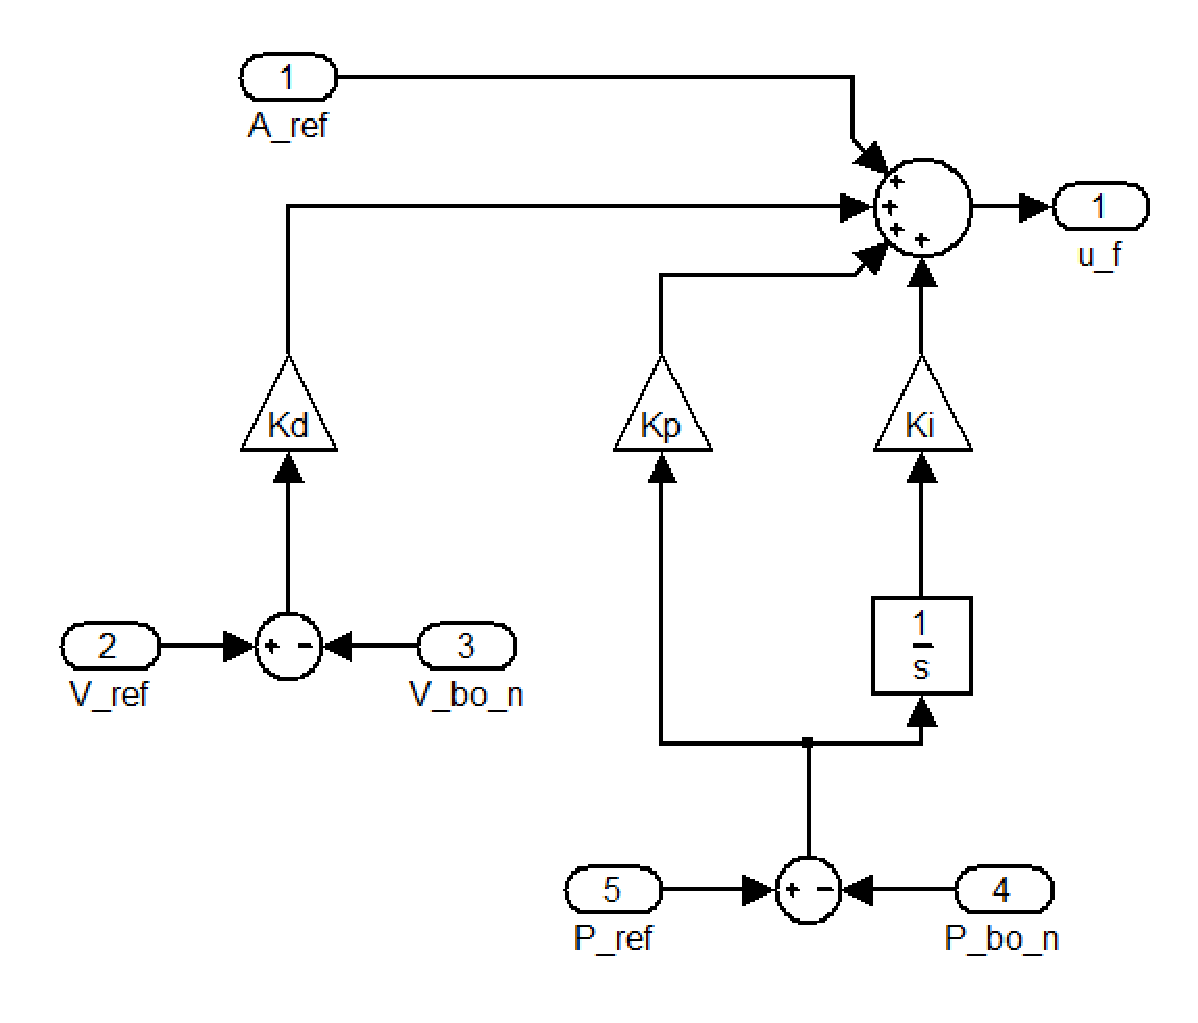
\includegraphics[width = .7\textwidth]{images/anlag_folgeregelung}
  
  \section{Modell des Fusionsfilters}
  
  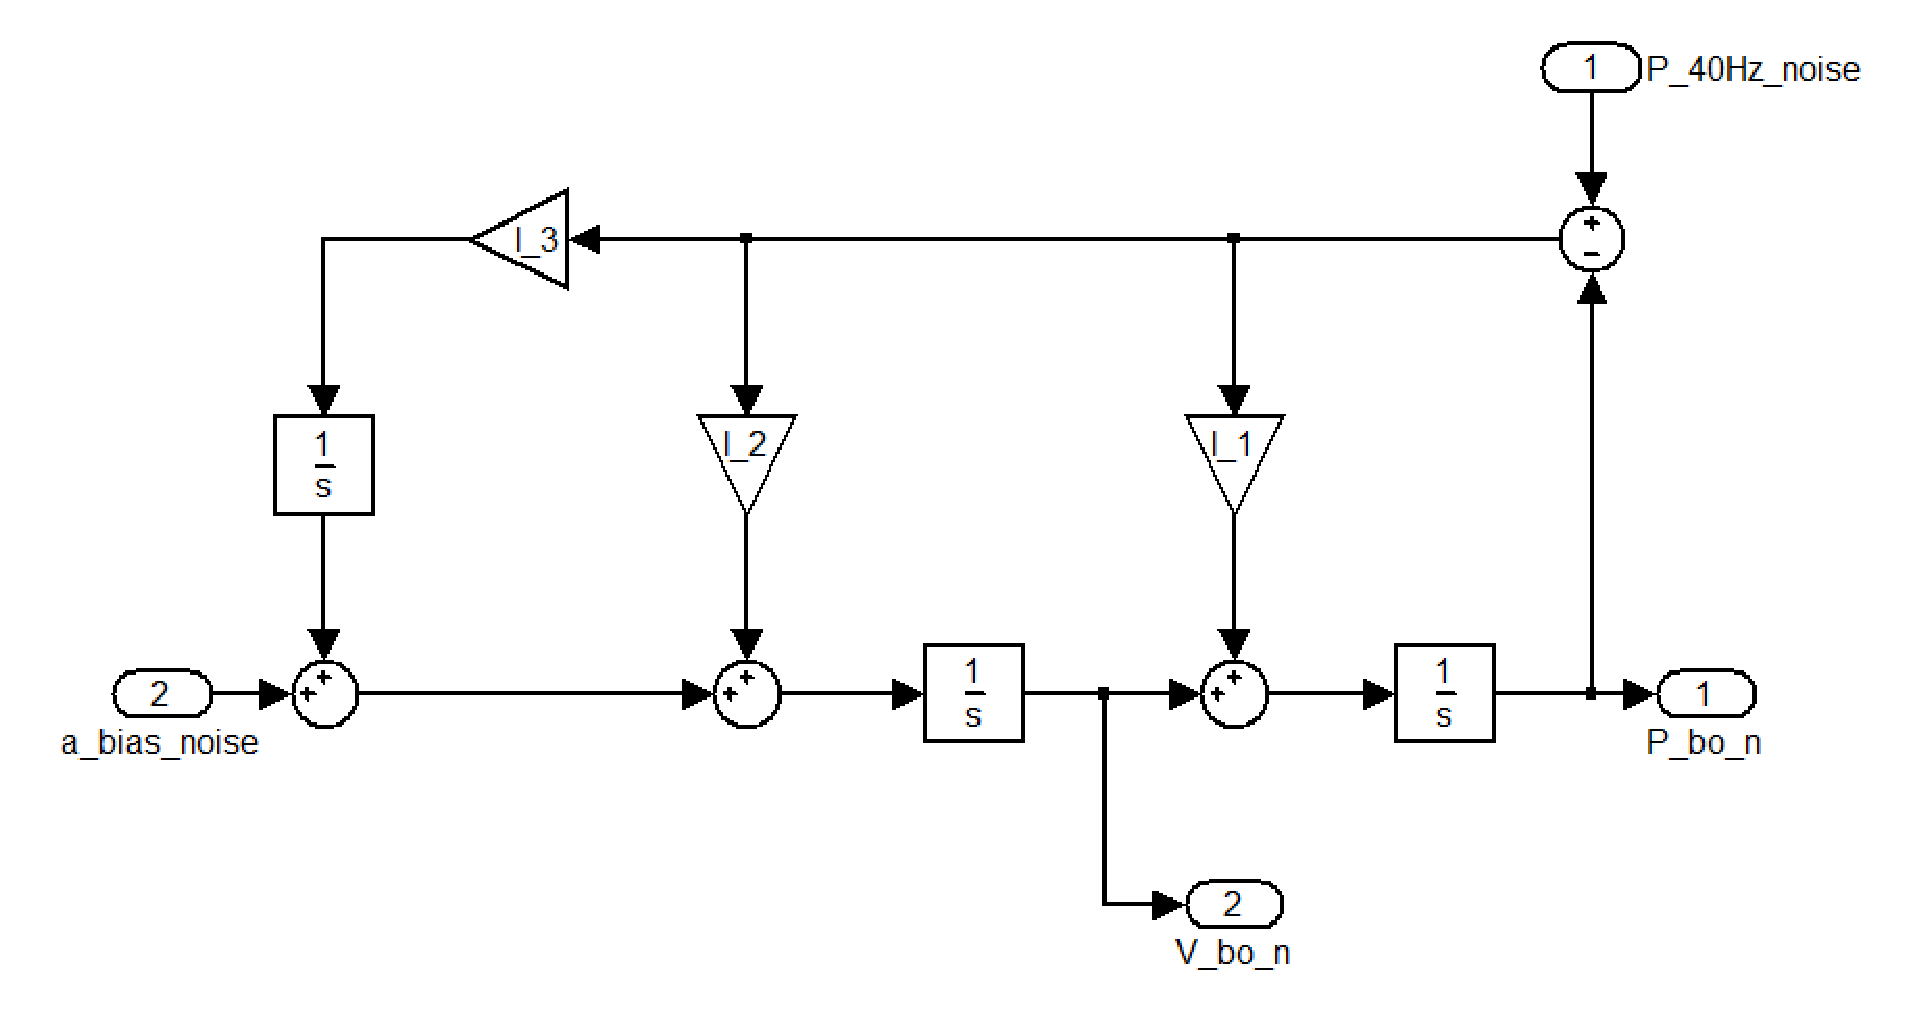
\includegraphics[width = .95\textwidth]{images/anlag_fusion}